\documentclass[10pt]{article}
\usepackage{geometry}                
\geometry{letterpaper}                   

\usepackage{graphicx}
\usepackage{amssymb}
\usepackage{epstopdf}
\usepackage{pdfpages}
\usepackage{amssymb, amsmath}
\DeclareGraphicsRule{.tif}{png}{.png}{`convert #1 `dirname #1`/`basename #1 .tif`.png}

\usepackage{amsrefs}

\graphicspath{ {./images/} }
\usepackage{caption}
\usepackage{subcaption}

\BibSpec{article}{%
  +{}{\PrintAuthors} {author}
  +{, }{ \textit} {title}
  +{, }{}{journal}
  +{, }{\textbf} {volume}
  +{ }{ \parenthesize} {year}
  +{, }{}{number}
  +{, }{}{pages}
  +{, }{}{publisher}
  +{, }{} {note}
}

%\title{Title}
%\author{Name 1, Name 2}
%\date{date} 

\begin{document}



\thispagestyle{empty}

\begin{center}

\includegraphics[width=5cm]{ETHlogo.eps}

\bigskip


\bigskip


\bigskip


\LARGE{ 	Lecture with Computer Exercises:\\ }
\LARGE{ Modelling and Simulating Social Systems with MATLAB\\}

\bigskip

\bigskip

\small{Project Report}\\

\bigskip

\bigskip

\bigskip

\bigskip


\begin{tabular}{|c|}
\hline
\\
\textbf{\LARGE{Insert Title Here}}\\
\textbf{\LARGE{...}}\\
\\
\hline
\end{tabular}
\bigskip

\bigskip

\bigskip

\LARGE{Name 1 \& Name 2}



\bigskip

\bigskip

\bigskip

\bigskip

\bigskip

\bigskip

\bigskip

\bigskip

Zurich\\
May 2008\\

\end{center}



\newpage


%%%%%%%%%% Table of content %%%%%%%%%%%%%%%%%

\tableofcontents

\section{Introduction}
The spreading of false news on social media has become a major issue in recent years. The uncontrolled circulation of biased and false information is eroding fundamental pillars of liberal societies as fair elections, free speech and public debate, thereby leading to increasing division and polarisation. This issue has provoked wide interest in the scientific community, leading to many interdisciplinary research projects (see for instance \cite{del2016spreading}, \cite{vosoughi2018spread}, \cite{lazer2018science}). However, ``false news science'' is still in its infancy and a solution to the false news problem is still far from sight. The aim of our project is to provide a small contribution to the understanding of this problem, via agent based models and simulations. With our model and code we aspire to answer specific cases of the following three broad research questions:
\begin{enumerate}
\item \label{intro:q1} How does network structure impact the spreading of news?
\item \label{intro:q2} What impact does the choice of initial spreaders have on the spreading of competing news? What is the best choice of initial spreaders when one aims to maximise cascade size? 
\end{enumerate}
Answers to these questions can be leveraged to curb the spreading of false news. For instance, insights on network topology can be used to build social networks with topologies which are more resilient to false news propagation. Similarly, understanding the impact of the choice of initial spreaders and what constitutes a ``good'' choice of initial spreaders can lead to a better understanding about how to counter false news. For example, one can use this understanding to improve the speed and breadth with/at which the information that the news is false spreads. \\

The model we employ and the questions above have been explored in various papers in the literature. Our model is a refinement of the threshold model originally introduced by Granovetter in \cite{granovetter1978threshold}. The model was given a decisive boost by the work of Watts \cite{watts2002simple}, who introduced it to the network science community. In \cite{watts2002simple}, Watts uses percolation theory techniques in order to estimate cascade sizes. Since the work of Watts, much research has been dedicated to extending the threshold model and exploring its relationship with the SIR model for epidemic spreading (see e.g. \cite{ran2020generalized} and \cite{dodds2004universal}). \\

The impact of network topology on the spreading of news has also been intensively studied in the literature. Watts characterised the conditions for large cascades to happen as a function of the degree distribution of the network \cite{watts2002simple} and simulated the case where the degree distribution is uniform. Singh et al. \cite{singh2013threshold} investigated the effect of network topology on cascade sizes, by studying a real high school network. Moreover, the authors of the aforementioned paper explored how the average connectivity of a network impacts cascade sizes. Their experiment and results resembles our own below.\\  

Finally, the impact of the initial choice of spreaders, the number of initial spreaders and the ``stubbornnes'' of initial spreaders has been thoroughly investigated by many research papers. The framework surrounding these research projects has often been the spreading of innovation or the attempt to maximise the marketization of products, rather than the attempt to minimise the spreading of false news. However, most of the insights transfer without much change. In maybe the leading paper of this field \cite{kempe2003maximizing}, Kempe et al. propose a greedy algorithm to select a set of initial spreaders which maximises cascade size in a threshold model. In this project, we implemented the algorithm proposed by Kempe et al. However, its performance was not remarkably superior than other simpler methods of selecting initial spreaders. Work by Singh et al. \cite{singh2013threshold} explores, via percolation theory methods, how cascades size varies as we vary initial fraction of spreaders. In the above papers the framework only treats the spread of one innovation/information. Xie et al. \cite{xie2012evolution} extend the model to allow for competing information within a network. Their focus is understanding how committed minorities can influence opinions of flexible majorities. \\

Our project is an attempt to blend together some of the insights and models contained in the literature above. In fact, both for our model and our experiments we have taken much inspiration from some of the aforementioned papers. \\

This report is structured as follows. In section 2, we present our model of news spreading in a social network. In section 3, we validate our model by investigating its behaviour when we change the parameters. In section 4, we illustrate results of a simulation aimed at answering question \eqref{intro:q1} in a specific case. Section 5 has analogous content focusing on question \eqref{intro:q2}. Finally, section 6 concludes.

\section{The model}
We fix a directed graph $G = (V,E)$. Our goal is to model the diffusion of news within this directed graph. To each node $v \in V$, we associate two sets of nodes: (i) the set $P(v)$ of nodes with an edge directed towards $v$ (i.e. $w \rightarrow v$ for $w \in P(v)$), which we call $v$'s \textbf{information providers}; (ii) the set $R(v)$ of nodes with an edge directed from $v$ towards them (i.e. $v \rightarrow w$ for $w \in R(v)$), which we call $v$'s \textbf{information receivers}. Each node $v$ can be in three states:  (i) \textbf{ignorant}: $v$ has not heard of the news yet (i.e. no information provider of $v$ is active); (ii) \textbf{inactive}:  $v$ has heard about the news but has not yet activated (i.e. at least one information provider of $v$ is active but $v$ is not active); (iii) \textbf{active}: $v$ has heard about the news and has activated  (i.e. at least one information provider of $v$ is active and $v$ is active). 
The idea is that an active node shares the news with his neighbours, an inactive node knows about the news but does not share it and an ignorant node does not know about the news. \\

How do nodes become active? Our model is based on the following simple principle: the probability of a node $v$ becoming active increases as more and more of his information providers become active. More precisely, each node $v$ gives a weight $r_{v,w}$ to all his information providers $w \in P(v)$. These weights should satisfy $\sum_{w \in P(v)} r_{v,w} = 1$. The value of $r_{v,w}$ represents the influence that information provider $w$ has on the decision of $v$ to become active. This model belongs to a well known class of models for innovation diffusion called threshold models \cite{watts2002simple}. \\

The activation dynamics run as follows. First, each node $v$ chooses a threshold $\phi_v \in [0,1]$ and an independence parameter $\alpha_v \in [0,1]$ via the uniform distribution; the threshold represents the weighted fractions of $v$'s information providers which have to be active in order to activate $v$; the independence parameter is meant to model the fact $v$'s decision is not totally dependent on the actions of his information providers. Then, we fix a set nodes $A_0$, which are initially active. These nodes are the initial spreaders of a news $N$ which has sensation $\rho \in [0,1]$; the sensation parametrises how attractive a news is. For each time step $t$ the process unfolds as follows:

\begin{enumerate}
\item If $t = 0$ all nodes in $V \setminus A_0$ are ignorant and all nodes in $A_0$ are active.
\item If $t > 0$ every node computes his excitement score $E_v$ with respect to the news $N$, which is given by:
\begin{align*}
E_v\Big((r_{v,w})_{w \in P(v)}, \alpha_v \Big) =  (1-\alpha_v)\sum_{w \in P(v)} \delta_a(w)r_{v,w}
\end{align*}

where $\delta_a(w) = 1$ if $w$ is active and zero otherwise. Next,
\begin{enumerate}
\item Any ignorant node with an active neighbour becomes inactive.
\item We activate any node $v$ with an excitement score $E_v$ satisfying:
\begin{align*}
E_v\Big((r_{v,w})_{w \in P(v)}, \alpha_v \Big) \geq \phi_v(1-\rho).
\end{align*}
\item Any active nodes with an excitement score $E_v$ satisfying $E_v < \phi_v(1-\rho)$ becomes inactive.

\end{enumerate}
Moreover, we update the sensation of the news by setting $\rho_{t+1} = \rho_{t}e^{-ct}$ for some constant $c$. This models the fact that a news becomes less sensational with time.
\item The dynamics end when no nodes change state for one time step.
\end{enumerate}

The graph model we use is a scale free network constructed via the algorithm proposed in the networkx package. The weights $r_{v,w}$  placed on edges are computed as follows. Node $v$ gives a weight:
\[ r_{v,w} = \frac{d_{out}(w)}{\sum_{u \in P(v) }d_{out}(u)} \]
to information provider $w$. This models the fact that nodes with higher out degree (i.e. with more information receivers) are considered more influential than nodes with low out degree. \\

Our main object of study will be the cascade size of a given news $N$, which we denote by $C(N)$. For us, the cascade size is a number in $[0,1]$ computed as the ratio of active nodes over total nodes.

\section{Model evaluation}
In order to validate our model and understand the impact of the model parameters on outcomes we ran some simulations. We quickly recap the main objects in our model and their parameters (which are described in section 2):
\begin{itemize}
    \item Object: Agent; Parameters: threshold, independence, weights of incoming and outgoing edges. 
    \item Object: News; Parameters: sensation, decay.
    \item Object: Graph; Parameters: graph topology.
\end{itemize}
Concerning the News object we ran experiments where we varied the following parameters:
\begin{itemize}
    \item Decay parameter and sensation
\end{itemize}
Regrading the Agent object we executed experiments where we simultaneously varied the following parameters:
\begin{itemize}
    \item Threshold and sensation
    \item Independence and sensation
    \item Threshold and independence.
\end{itemize}
Finally, we ran a couple of experiments to determine how the number and choice of initial active agents impact the cascade size in our model.
Details on the all above experiments can be found in sections \ref{subsec:decay_sensation}-\ref{subsec:threshold_independence} below. The results of the experiments are shown in figure \ref{fig:phase_diagrams}. \\

The following remarks hold for all the experiments we ran.
\begin{itemize}
    \item If a parameter of the agents is varied in an experiment, its value is the same for all agents in the network.
    \item Parameters which are not considered in the experiment are sampled uniformly from the parameter space. The choice of uniform sampling prevents introducing biases in parameters which are not considered in the experiment.
    \item In all experiments (except ``decay parameter vs sensation'') the decay parameter of the news is set to 0 to prevent interference with the effect of the parameters that are considered.
    \item An experiment with a pair of parameters (e.g. a (threshold, sensation) pair in figure \ref{fig:threshold_sensation}) is executed multiple times to sample from different networks. With this we average out random effects in the results.
\end{itemize}

All experiments in figure \ref{fig:phase_diagrams} were executed on a network with 1000 agents and repeated 50 times.

\begin{figure}
    \centering
    \begin{subfigure}{0.48\textwidth}
      \centering
      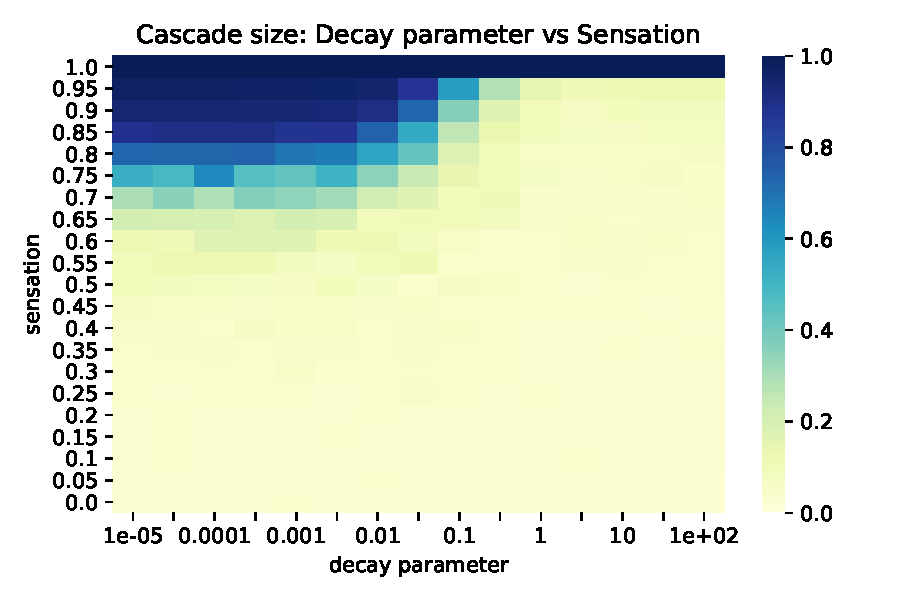
\includegraphics[width=0.95\textwidth]{images/decay_sensation.pdf}
      \caption{Cascade size for different decay rates and news sensations.}
      \label{fig:decay_sensation}
    \end{subfigure}\hfill
    \begin{subfigure}{0.48\textwidth}
      \centering
      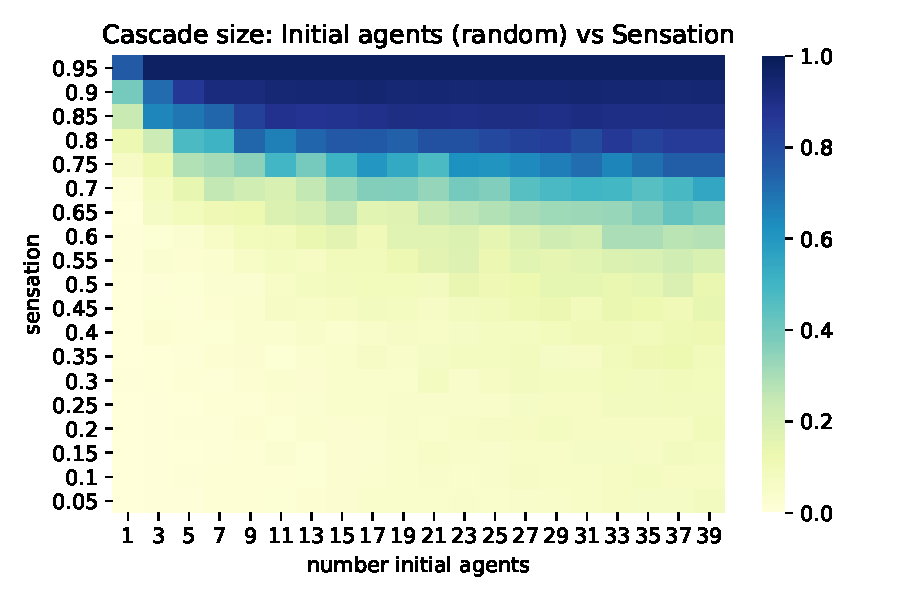
\includegraphics[width=0.95\textwidth]{images/initial_sensation_random.pdf}
      \caption{Cascade size for different number of initial active agents and news sensations. Here the initial active agents are chosen randomly.}
      \label{fig:initial_sensation_random}
    \end{subfigure}\\
    \begin{subfigure}{0.48\textwidth}
      \centering
      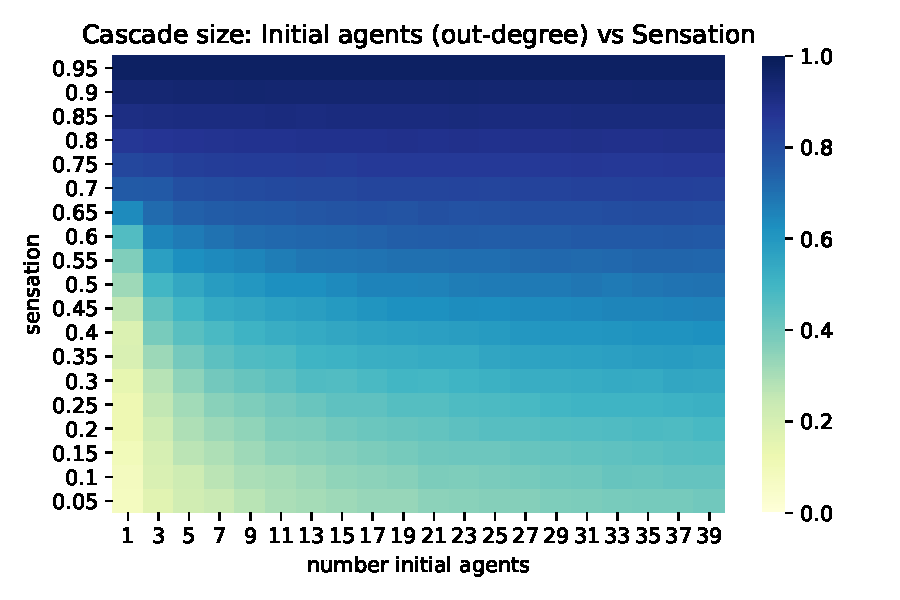
\includegraphics[width=0.95\textwidth]{images/initial_sensation_out_degree.pdf}
      \caption{Cascade size for different number of initial active agents and news sensations. Here the initial active agents are chosen by degree centrality.}
      \label{fig:initial_sensation_out_degree}
    \end{subfigure}\hfill
    \begin{subfigure}{0.48\textwidth}
      \centering
      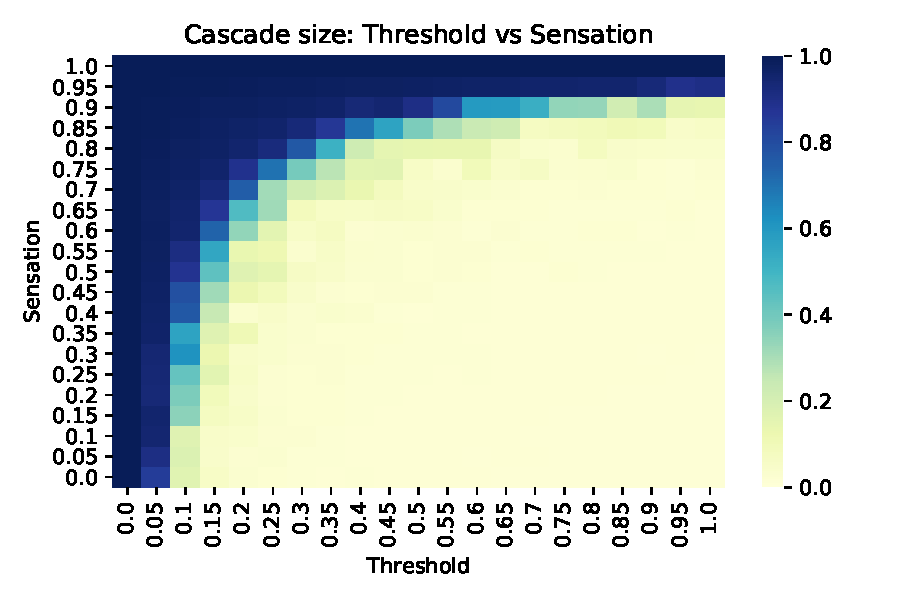
\includegraphics[width=0.95\textwidth]{images/threshold_sensation.pdf}
      \caption{Cascade size for different agent thresholds and news sensations.}
      \label{fig:threshold_sensation}
    \end{subfigure}\\
    \begin{subfigure}{0.48\textwidth}
      \centering
      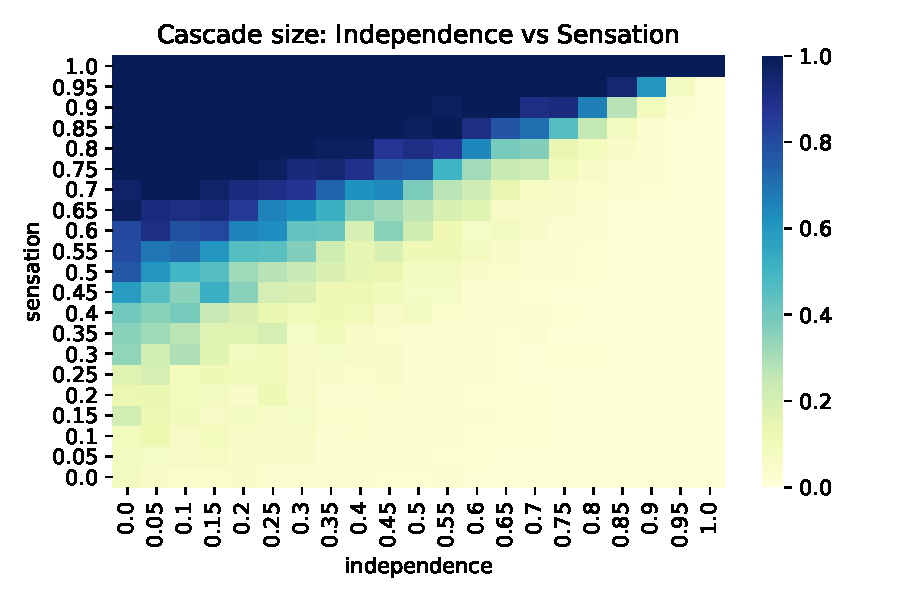
\includegraphics[width=0.95\textwidth]{images/independence_sensation.pdf}
      \caption{Cascade size for different agent independence values and news sensations.}
      \label{fig:independence_sensation}
    \end{subfigure}\hfill
    \begin{subfigure}{0.48\textwidth}
      \centering
      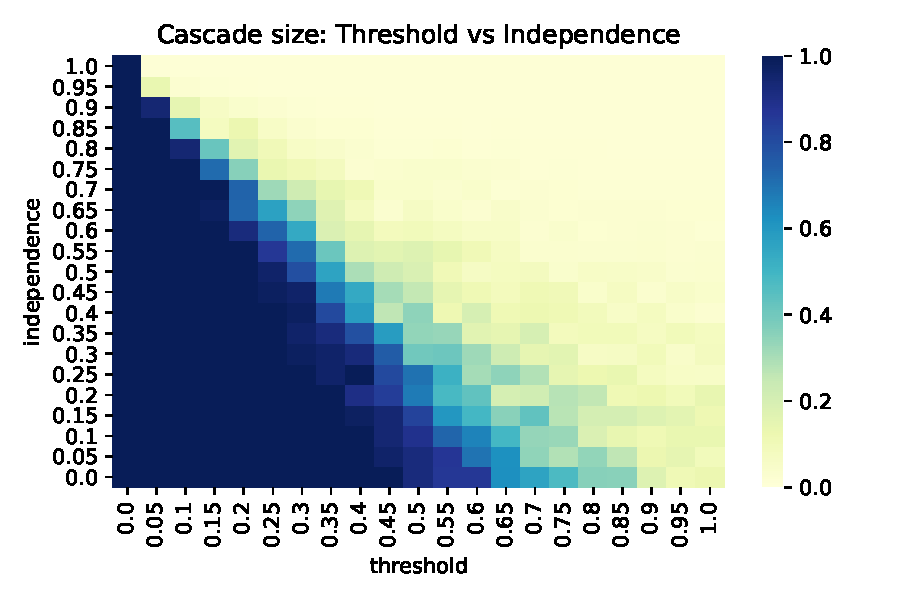
\includegraphics[width=0.95\textwidth]{images/threshold_independence.pdf}
      \caption{Cascade size for different agent thresholds and independence values for a news with a sensation of 0.8.}
      \label{fig:threshold_independence}
    \end{subfigure}
    \caption{Cascade size for different agent parameter values. All experiments were simulated with one news in the system. }
    \label{fig:phase_diagrams}
\end{figure}

\subsection{Decay parameter vs Sensation}\label{subsec:decay_sensation}
In this experiment we varied the decay parameter and the sensation parameter of the news; the results are shown in figure \ref{fig:decay_sensation}. Cascade sizes are higher for low values of the decay parameter and high sensations. This matches our expectations as news with high sensation should spread further and small values for the decay parameter allow the news to remain active in the system for longer. 

\subsection{Number of initial active agents vs Sensation}\label{subsec:inital_agents_sensation}
The results of the experiments are shown in figures \ref{fig:initial_sensation_random} and \ref{fig:initial_sensation_out_degree}. The number of initial active agents refers to the number of agents which are activated at the start of the simulations. In figure \ref{fig:initial_sensation_random} the initial active agents are chosen randomly and in figure \ref{fig:initial_sensation_out_degree} they are chosen according to the degree centrality. The results match our expectations. If more agents are activated at the start of the simulations, cascades are larger. However, we notice that the cascade size increases sub-linearly in the number of initial active agents when agents are activated randomly. For the activation according to the degree centrality we can not say something similar, as very few initial active nodes are necessary for the news to spread in the network, even for low sensations of the news.\\


\subsection{Threshold vs Sensation}\label{subsec:threshold_sensation}
Two fundamental parameters of the model are thresholds and news sensation.
In this experiment we vary both parameters and plot cascade sizes as a function of these parameters. Results are shown in figure \ref{fig:threshold_sensation}; they match our expectations. The news spreads in the region of high sensation and low thresholds.
Two interesting phenomena can be observed. First, the model displays a remarkable phase transition as the parameters vary: either the news spreads completely in the network, or it does not spread at all.
This result is in accordance with most spreading models. Second, the shape of the boundary of this phase transition is not linear. In particular, at low threshold levels, a small increase in thresholds requires a large increase in sensation in order to maintain the same cascade size. 

\subsection{Independence vs Sensation}\label{subsec:independence_sensation}
In this experiment we vary the agents independence parameter and the news sensation and plot cascade sizes for different choices of these parameters. Results are shown in figure \ref{fig:independence_sensation}. In the figure we see that the news spreads in the region of low independence and high sensation. This matches our expectations as the lower the independence of the agents the more susceptible they are to the influence of the providers.
In this plot phase transitions are less pronounced. For low independence and medium sensation, the model allows for ``medium'' cascade sizes. 

\subsection{Threshold vs Independence}\label{subsec:threshold_independence}
For this experiment we looked at the relation between the threshold and independence values of the agents for a news with sensation 0.8. From the previous experiments conducted (i.e. results in figure \ref{fig:threshold_sensation} and figure \ref{fig:independence_sensation}) we would expect cascade sizes of one for thresholds below $\approx 0.3$ and independence below $\approx 0.6$. In other words, we expect the square $[0,0.3]\times [0,0.6]$ in the plane with $x$ axis being threshold values and $y$ axis being independence values to have cascade sizes of one. This expectation is confirmed by the results in figure \ref{fig:threshold_independence}. This shows our model acts coherently when parameters are changed and hence hints at the correctness of our code implementation.

\section{Network Structure}
The first question we answer with our model concerns the impact of network structure on cascade size.
To formulate our question precisely, let us define the centralisation of a network to be the average number of information providers a node possesses. 
% Even better is the entropy of the probability distribution over information providers.
Let us also define the density of a network to be the number of edges in the network divided by the number of all possible edges (i.e. $n\choose{2}$ if the network has $n$ nodes). Our aim is to understand how cascade size varies as a function of density and centralisation of a network.  \\

In order to address the above question we build networks $G(k,z)$, where $k \in \mathbb{N}$ is a proxy for density and $z \in [0,1]$ a proxy for centralisation. In greater detail, we start off with $n$ nodes $v_1, \ldots ,v_n$, which we arrange in a circle. For each node $v_i$, we add two edges $v_i \rightarrow v_{i+1}$ and $v_{i+1} \rightarrow v_i$. This gives us a double directed cycle between all the nodes. This is our "base graph", which we call $G_b$. Starting from $G_b$ we build graphs $G(k,z)$ using the following algorithm: \\

\begin{figure}[h]
\centering
\begin{subfigure}{.5\textwidth}
  \centering
  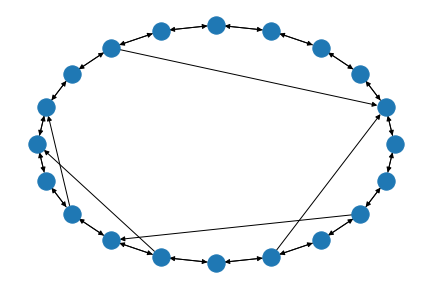
\includegraphics[width=.9\linewidth]{example2}
  \caption{$z = 0$}
\end{subfigure}%
\begin{subfigure}{.5\textwidth}
  \centering
  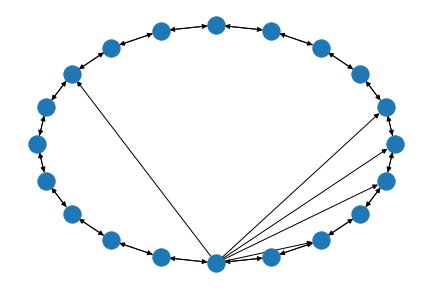
\includegraphics[width=.9\linewidth]{example8}
  \caption{$z = 1$}
\end{subfigure}
\caption{Graphs $G(k,z)$ with $k = 5$ and $z$ as above}
\label{fig:test}
\end{figure}

For $a = 1, \ldots, k$ repeat the following:
\begin{enumerate}
\item If $a = 1$, choose a random node $v_i$, the information provider, and a random node $v_j$ not in $R(v_i)$, the information receiver. Then, add the edge $v_i \rightarrow v_j$ to $G_b$. That is, we make $v_i$ an information provider of $v_j$.
\item For $a > 1$, let $v_i$ be the information provider selected in round $a-1$. With probability $z$, we keep $v_i$ as information provider for round $a$ and select a random node $v_j$ not in $R(v_i)$ as information receiver. Then, we add the edge $v_i \rightarrow v_j$. With probability $1-z$, we choose a random node $v_k$ from the set of all nodes except $v_i$ as information provider. Then, we select a random node $v_j$ not in $R(v_k)$ as information receiver and add an edge $v_k \rightarrow v_j$.
\item If at some point of the procedure above we select as information provider a node $v_i$ satisfying $R(v_i) = V\setminus {v_i}$ (that is, all other nodes are information receivers of $v_i$) we simply discard this node, select another node at random as information provider and continue as above.
\end{enumerate}


What is the idea behind the construction above? Let's explore the limit cases. If $z = 1$, then we always choose the same node as information provider to add new edges. This models a network where everyone listens to the same information source (i.e. a centralised network). If $z = 0$, we always choose a random new node as information provider. Therefore, the network has plenty of nodes providing information to each other (i.e. information provision is decentralised). The base graph $G_b$ built in the beginning is to assure that the final graph we obtain is connected.  \\

Once we have gone through the above procedure and constructed the graph $G(k,z)$, we give weights to edges as described in the model section.\\

In Figure \ref{fig:graph structure} we plot the results of our simulations as we vary the parameters $k$ and $z$ for news sensations of 0.9 and 0.5.
For the simulations the agent thresholds and independence are sampled from uniform distribution and one agent is initially activated randomly (i.e. $|A_0| = 1$). Our graph had $1000$ agents. As always we ran multiple simulations of each graph and average out over the results.\\

\begin{figure}[h]
\centering
\begin{subfigure}{.5\textwidth}
  \centering
  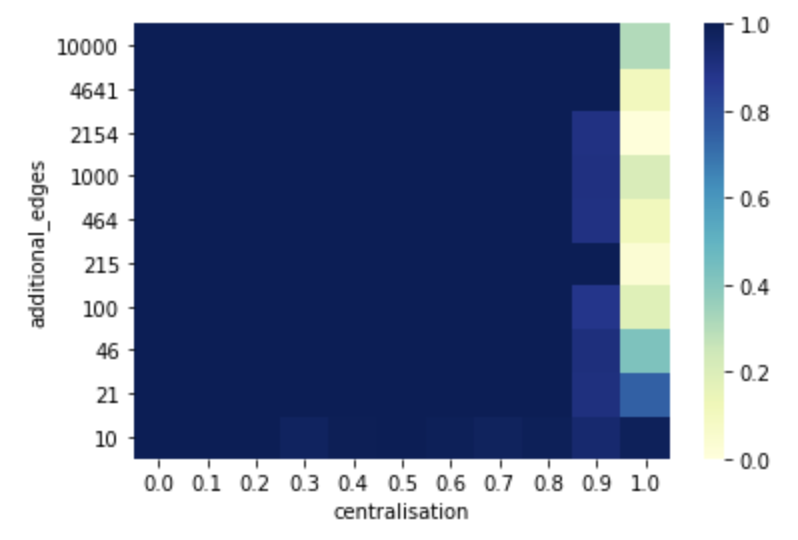
\includegraphics[width=.9\linewidth]{heatmap_graph_structure_09}
  \caption{sensation = 0.9}
  \label{fig:graph structure:sub1}
\end{subfigure}%
\begin{subfigure}{.5\textwidth}
  \centering
  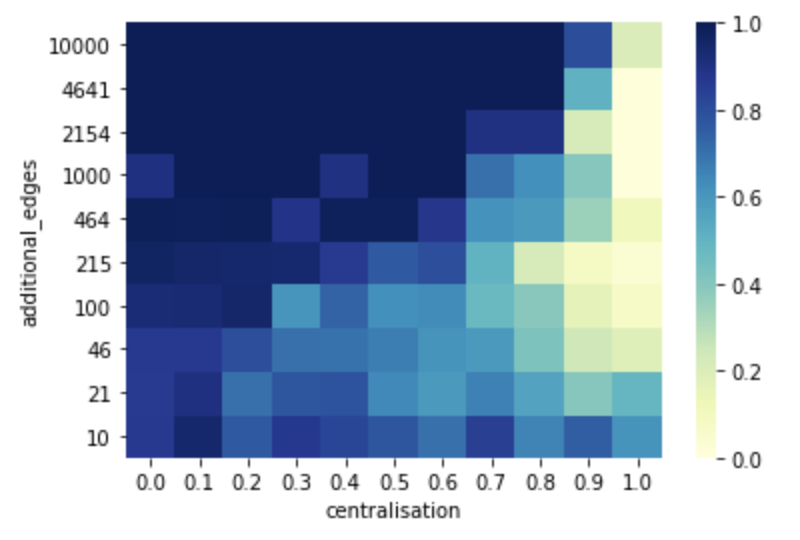
\includegraphics[width=.9\linewidth]{heatmap_graph_structure_050}
  \caption{sensation = 0.5}
  \label{fig:graph structure:sub2}
\end{subfigure}
\caption{Heatmaps for centralisation vs number of additional edges of a graph}
\label{fig:graph structure}
\end{figure}

From the results in figure \ref{fig:graph structure} we observe that cascade sizes are higher in dense decentralised networks and lower in any form of centralised network. This result makes intuitively sense since if every node is listening to the same information provider and that provider does not activate, all his listeners will not activate too. On a model standpoint, this is a consequence of the way we selected the edge weights (or influence). In particular, nodes give more weight to higher out-degree nodes when deciding to activate or not. In a decentralised network, most nodes have the same out degree and so all nodes exert similar influence. In a centralised network, few nodes have huge degrees and exert massive influence and most other nodes do not. Hence, it is very unlikely that a news shared by a random node would spread in such a network. \\

\section{Initial spreaders and multiple news}
The second question we address concerns the impact of initial spreaders on competing news. Assume we have two competing news $N_1, N_2$. At time $t = 0$, we activate the nodes $A_0^1$ with respect to news 1 and run the dynamics described in section 2. At time $t = s$, we activate nodes $A_0^2$ with respect to news 2. At this point two news are competing for attention within the network. The dynamics of spreading are the same as those described in section 2, with the following two additional rules:
\begin{enumerate}
\item Any node $v$ can be active with respect to a unique news at any given time. However, he can shift from active with respect to one news to active with respect to the other.
\item Let $E_v^1, E_v^2$ be the excitement scores of node $v$ with respect to $N_1$ and $N_2$. If both excitement score surpass the threshold for activation, agent $v$ activates with respect to the news with the higher excitement score.
\end{enumerate}
We used the above scenario to address the following questions:
\begin{enumerate}
\item How does the difference in final cascade size of the two news vary as we vary the sensation parameters?
\item How does the choice and size of the initial active set $A_0^{i}, \ i =1,2$ impact the final cascade sizes of the two news?
\item How does the time delay in activation $s$ of $N_2$ with respect to $N_1$ impact the cascade sizes of the two news?
\end{enumerate}

For the first question our result can be seen in figure \ref{fig:sens_vs_sens}. Here, we plot the difference is cascade size between two news as we vary their sensation parameter. Initially we activate 5 random agents per news. A value of -1 corresponds to total spread of news 2 over news 1 and a value of 1 to the converse situation.  First we observe that since we have a symmetrical situation, the plot is also symmetric. Next, we note that if both sensations are below a certain value, $0.4/0.5$ approximately, then neither of the news will manage to dominate the whole network and therefore the difference between the two cascade sizes will be close to 0. However, for the opposite case, when both news have a relative high sensation parameter, it is much more likely that the one with a higher sensation is going to spread across almost the whole structure, leading to a very high final cascade size. This is intuitively connected to the fact that a news can activate an already active (with respect the the other news) agent only if both the threshold and the excitement score of the other news are surpassed. Therefore, only for low sensations we get that the threshold value has the effect to stop a news from prevailing.
\begin{figure}
\centering
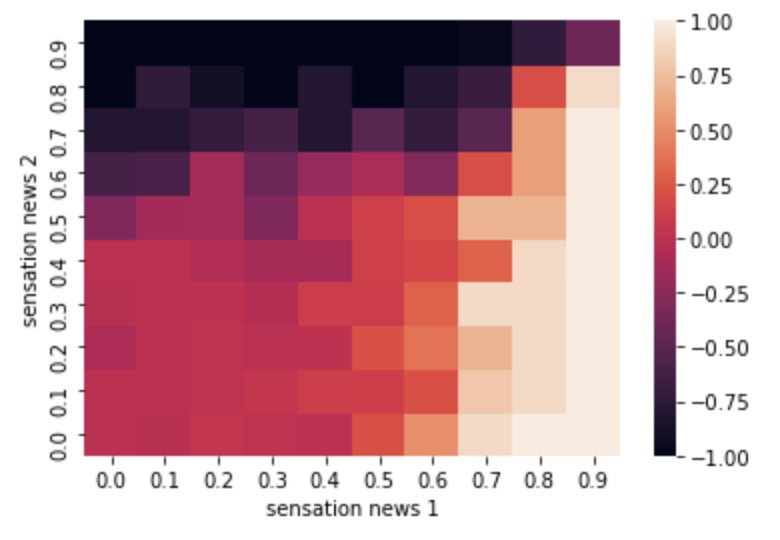
\includegraphics[width=.7\linewidth]{images/sens_vs_sens.png}
\caption{Difference in fraction cascade sizes of two news as sensation varies.}
\label{fig:sens_vs_sens}
\end{figure}
We deduce from this that differences in sensation in not very sensational news do not lead to large differences in spreading, while the effect is opposite for highly sensational news. \\

Concerning the second question above, our results are illustrated in figure \ref{fig:set_type_comparison}. Here, we did the following: we activated $|A_0^{1}| = 5$ degree central nodes for news 1 and different quantities of initial nodes for news 2 (see figure), chosen from the remaining nodes not in $A_0^1$. We observe that activating initial agents with degree centrality generates vastly larger cascades with respect to random activation. For instance, activating 200 random agents for news 2 is worse than activating the 20 degree central agents. We see similar results for the case of 500 random agents vs 50 degree central agents. However, as we increase the number of initially activated agents we expect the difference to be less pronounced. \\
\begin{figure}
\centering
\begin{subfigure}{0.475\textwidth}
  \centering
  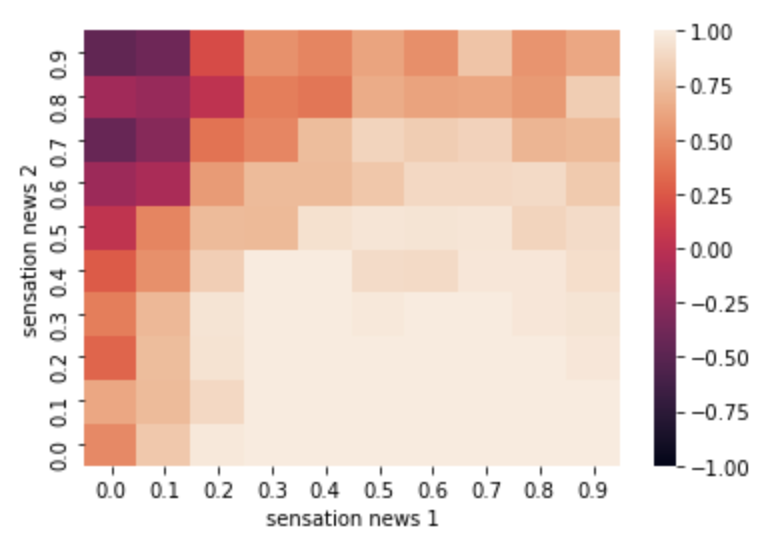
\includegraphics[width=.9\linewidth]{images/asize200.png}
  \caption{$|A_0^2|=200$ random nodes}
  \label{fig:set_type_comparison:sub1}
\end{subfigure}
\hfill
\begin{subfigure}{0.475\textwidth}
  \centering
  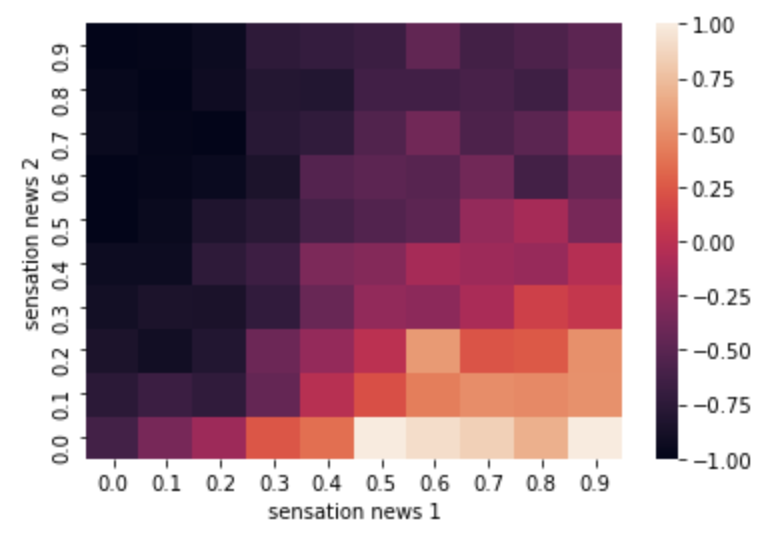
\includegraphics[width=.9\linewidth]{images/asize500.png}
  \caption{$|A_0^2|=500$ random nodes}
  \label{fig:set_type_comparison:sub2}
\end{subfigure}
\vskip \baselineskip
\begin{subfigure}{0.475\textwidth}
  \centering
  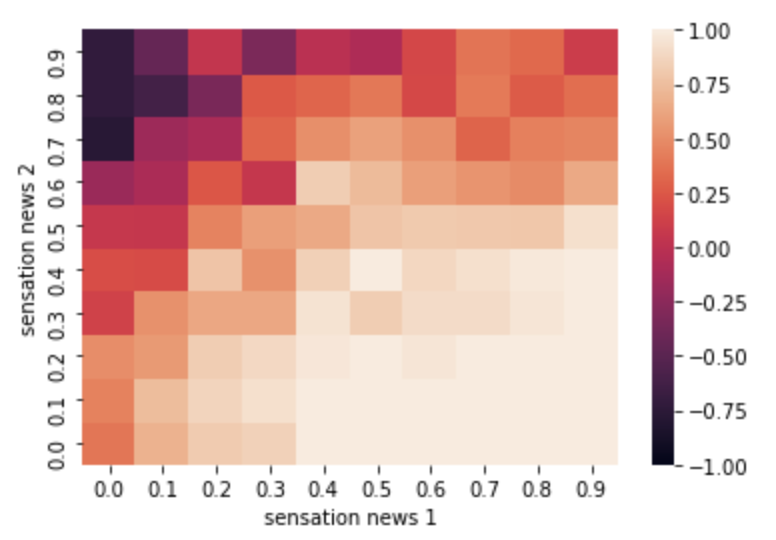
\includegraphics[width=.9\linewidth]{images/kset20.png}
  \caption{$|A_0^2|=20$ degree central nodes}
  \label{fig:set_type_comparison:sub3}
\end{subfigure}
\hfill
\begin{subfigure}{0.475\textwidth}
  \centering
  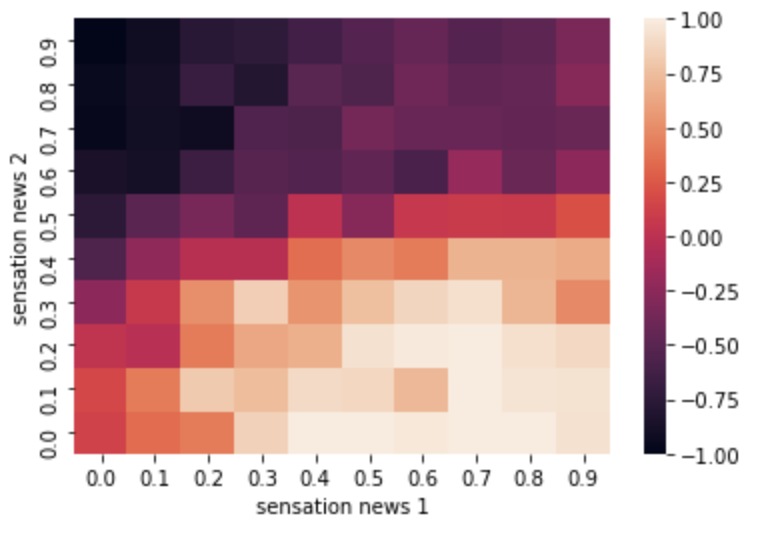
\includegraphics[width=.9\linewidth]{images/kset50.png}
  \caption{$|A_0^2|=50$ degree central nodes}
  \label{fig:set_type_comparison:sub4}
\end{subfigure}
\caption{Difference in fraction of nodes covered for different starting sets (1000 agents total)}
\label{fig:set_type_comparison}
\end{figure}

But, is degree centrality the best notion of ``good'' initial active agents? That is, can a different choice of an algorithm for initial starting agents perform better than degree centrality in terms of cascades size? Let us define a function $\sigma$ mapping a subset of nodes $A$ to the expected value of the cascade size of $A$ in our threshold model, denoted $\sigma(A)$.
Kempe et al. \cite{kempe2003maximizing} show that maximising the function $\sigma$ is an NP-hard problem by reducing it to the Set Cover problem. Next, the authors prove that the function $\sigma$ proposed above is submodular (i.e. exhibits decreasing marginal returns) and leverage this property to construct a greedy algorithm which, given an integer $k$, can compute a $k$-set of nodes whose influence is a $(1-1/e-\epsilon)$-approximation of the maximum possible influence that can be achieved with a set of size $k$ in the network. The $\epsilon$ stems from part of the greedy algorithm, where graphs are sampled from the original network by choosing one edge for each node at random taking in account the edges weight. Kempe et al. prove that for a given set $A$, the expected number of nodes influenced by $A$ when running the linear threshold model is the same as the expected number of nodes reachable by set $A$ in the sampled graph. As one can make arbitrarily many samples $\epsilon$ can become arbitrarily small.\\

In this project, we implemented this greedy algorithm and compared its results in choosing ``good'' initial active agent sets with the much simpler degree centrality algorithm. As can be seen in figure \ref{fig:greedy} we got somewhat surprising results: The ``dot''-nodes show the resulting cascade size when taking the solution of the greedy algorithm or the most degree central set as the initial set. The greedy solution performs mostly a bit worse. This is a contrast with the results of Kempe et al \cite{kempe2003maximizing}, who showed that the solution of the greedy algorithm performed much better than choosing the initial set by means of degree centrality. The additional ``plus''-nodes in figure \ref{fig:greedy} show how the greedy algorithm would expect the two solutions to perform, i.e. we use the $\epsilon$-approximation mentioned above, that approximates the expected number of nodes influenced, and apply it to the solutions of both the greedy algorithm but also the the most degree central set. As can be seen, the greedy algorithm expects it's solution to perform much more similarly to the degree central solution than it actually does. This might be one reason, why the greedy algorithm did not provide the results similar to the ones of Kempe et al. Other reasons behind the difference might be the following:
\begin{enumerate}
    \item[1.] The greedy implementation is still quite slow so the experiment was done with only 100 agents and with not enough samples. There could be different result for larger networks.
    \item[2.] Since we augmented our model with additional parameters, such as news sensation and agent independence, the greedy approximation might need to take them into consideration.
    \item[3.] Our model is directed where the standard threshold model is not.
    \item[4.] We might have made a mistake in the implementation.
\end{enumerate}
Because degree centrality performed better than the greedy approximation and because it is much faster to compute, it was used as a notion for good initial active sets to answer question 3. \\

\begin{figure}
\centering
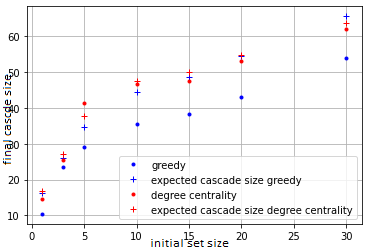
\includegraphics[width=.6\linewidth]{images/greedy.png}
\caption{Example of actual and expected (by greedy algorithm) cascade size of the same news in a 100 agent network with different starting sets (5 samples per starting set)}
\label{fig:greedy}
\end{figure}

For the third question, we consider a scenario where the sensation of the news does not decay over time. We study the difference in the cascade size of two news when the model reaches equilibrium (i.e. no more state changes for agents). Our experiment aims at understanding the effect of an initial delay on the spreading of a given news. Practically it runs as follows. First, the news 1 ($N_1$) is launched from the highest degree node, so $|A_0^1|=1$. Then after a delay of $s$ time steps the news 2 ($N_2$) is launched as a "counter" from the 5 highest degree nodes apart from the node in $A_0^1$. Additionally, the independence of all starting nodes in $A_0^1$ and $A_0^2$ is set to $1$, as they are starting $N_1$ or $N_2$ so they are not influenced by any other news. \\

As seen in figure \ref{fig:two_news_delays_no_decay}, the cascade size varies between no delay $s=0$ and positive delay $s>0$. However, we notice almost no difference between different values of positive delay. This could be explained by a combination of the following heuristic arguments: (i) Agents activated in the first step have in general higher excitement scores with respect to news 1 than agents activated in later rounds. This is because more of their neighbours are likely to be active, since their activation is positively correlated with that of their neighbours. As a result, their opinion is harder to flip with respect to the opinion of agents which activate in later rounds. (ii)
The threshold of an active agent with respect to news 1 is essentially higher for news 2, since news 2 now has to overcome not only the threshold of the active agent but also its excitement score for news 1. Moreover, if this agent was activated in the first round, the threshold for news 2 is on average even higher by what said in the first point.  (iii) Since the first active agent for news 1 is the most degree central agent, it is likely that most of the nodes news 1 activates are activated in the first step. Indeed, an agent with high degree has, in our model, high influence on its neighbours.
Moreover, nodes with low thresholds are activated in the first step, leaving nodes with higher thresholds to be activated in later steps. These arguments illustrates how, on average, more nodes should be activated with respect to news 1 in the first step of the dynamics than in later steps. Combining the three points above we observe that: most nodes active for news 1 are activated in the first step and nodes activated in the first step are the hardest to flip for news 2. Moreover, in subsequent steps, fewer nodes will activate for news 1 and they will be easier to flip for news 2 by what said in (i). Hence, the nodes activated in latter steps will have a marginal impact on the size of news 1's cascade. This explains why we see no difference between $s= 1$ and $s=8$ in figure \ref{fig:two_news_delays_no_decay}.

\begin{figure}[h!]
\centering
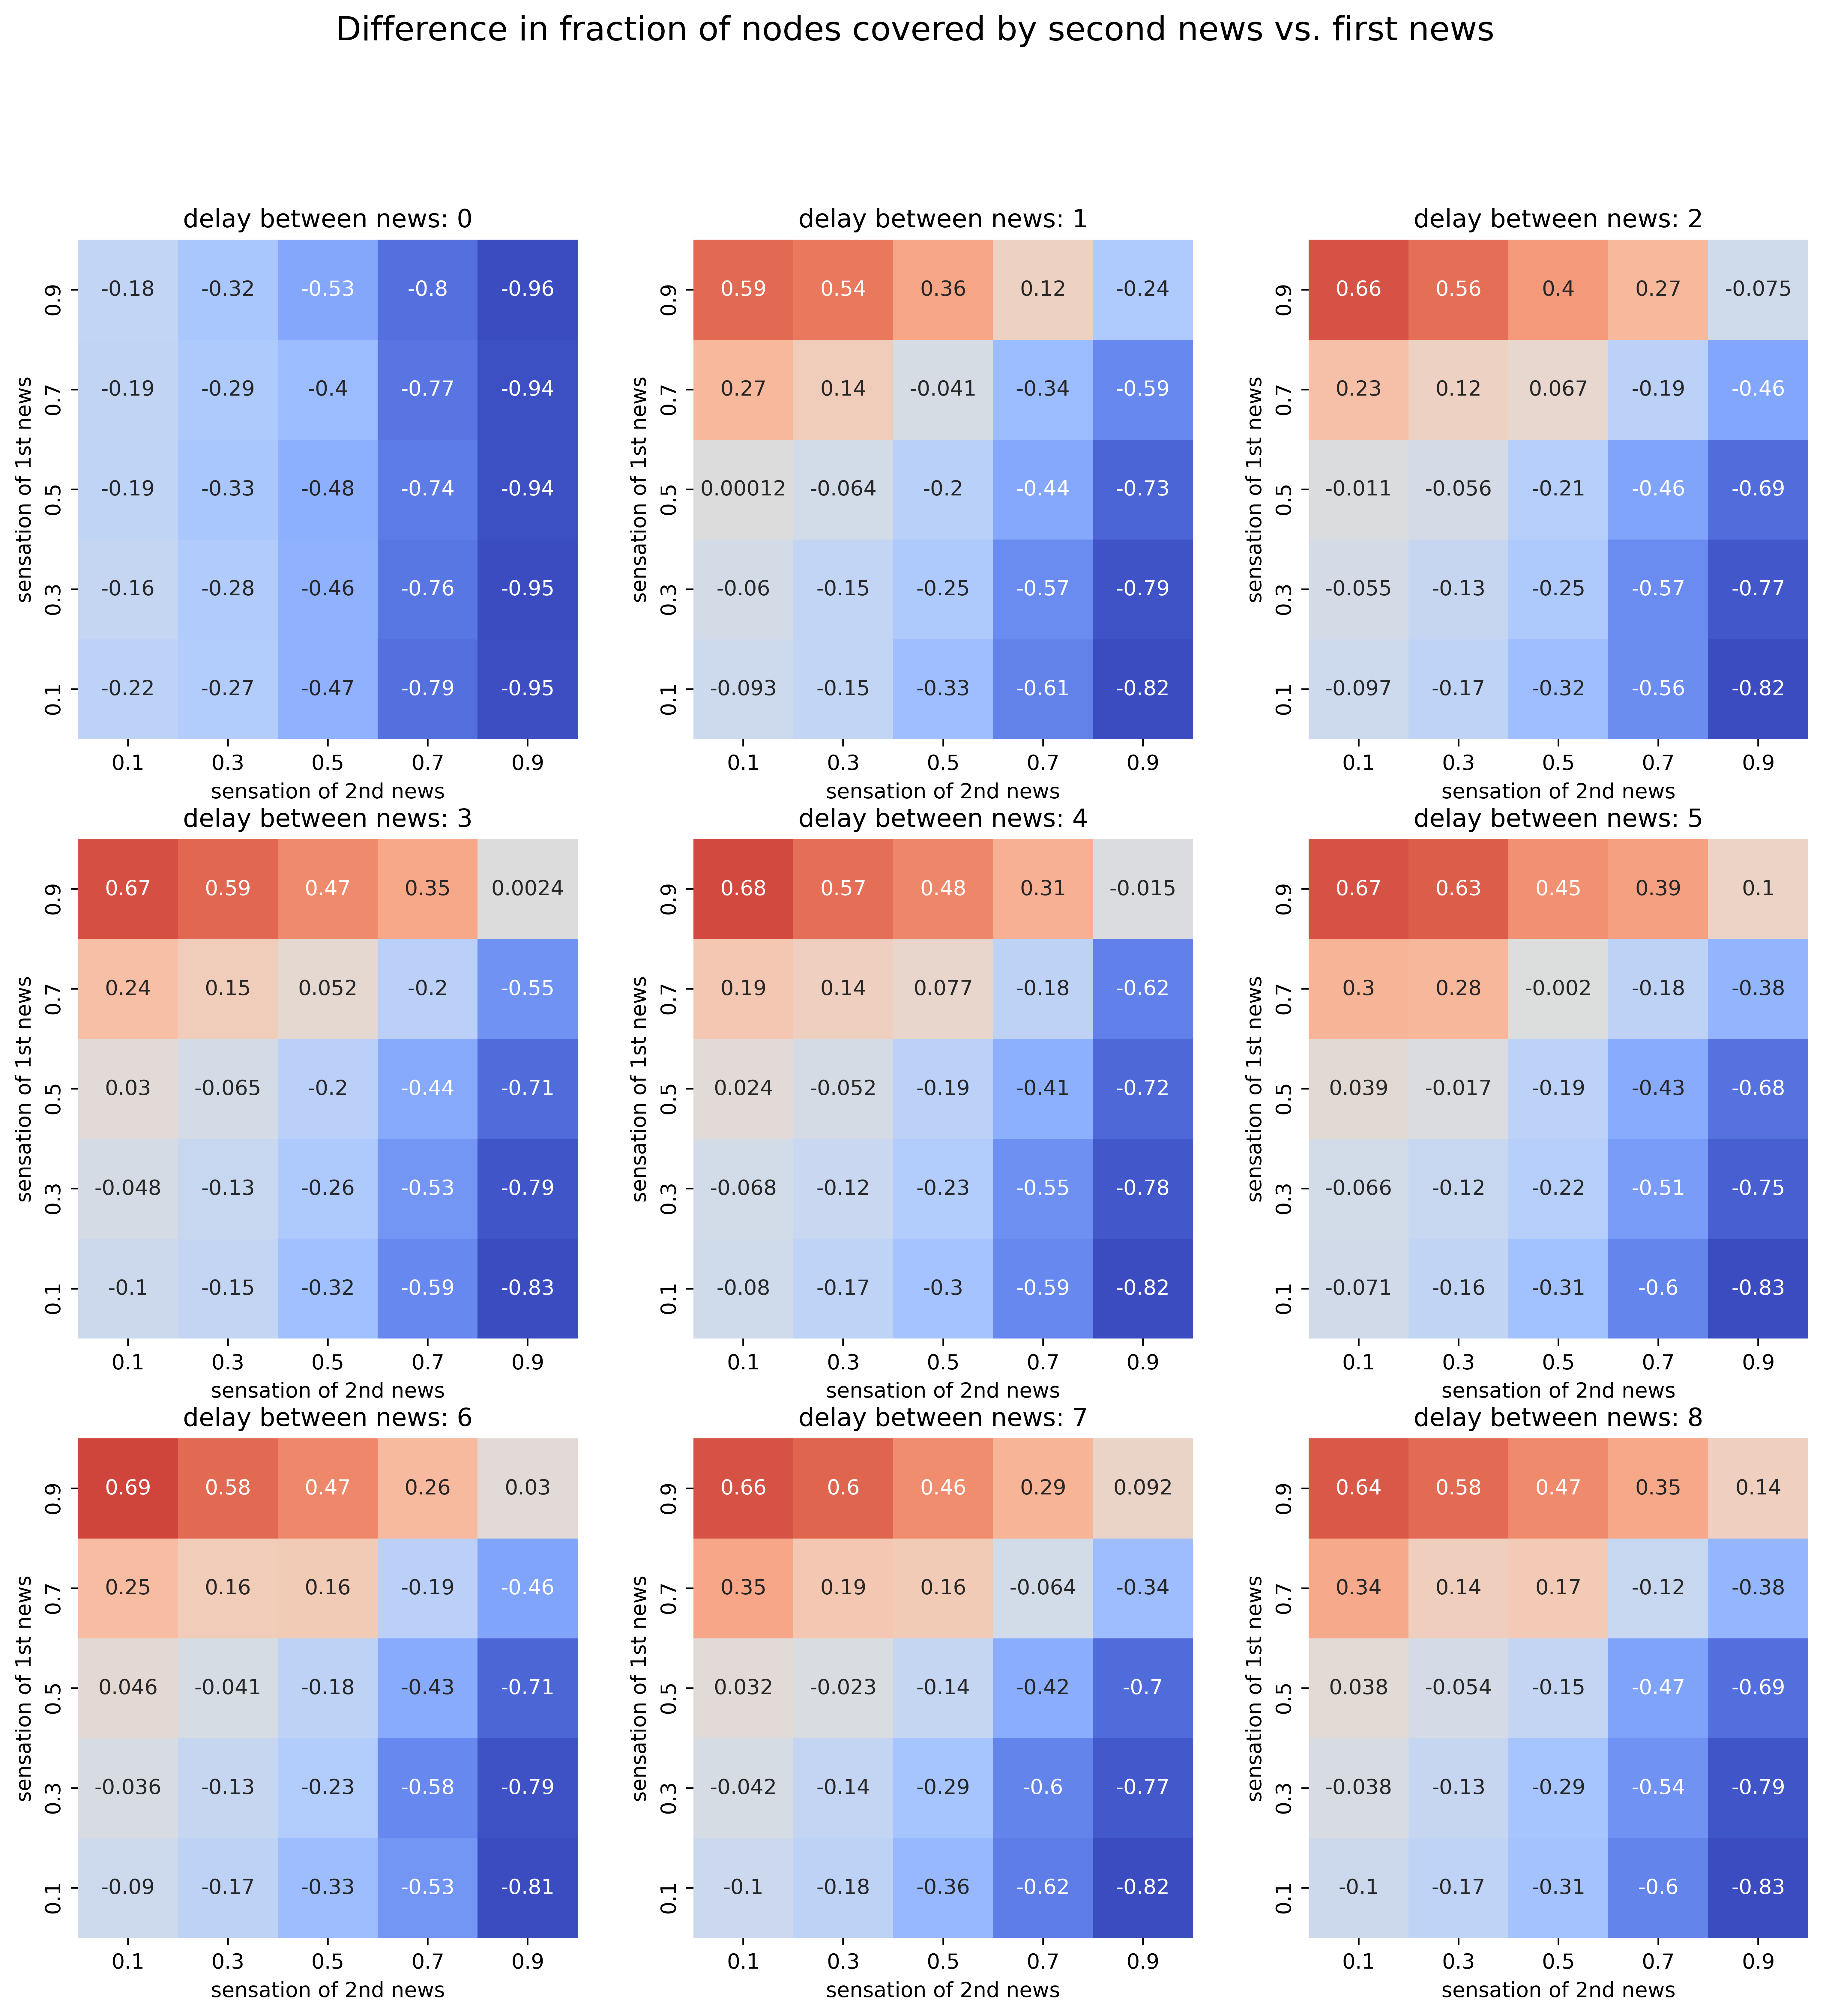
\includegraphics[width=1.0\linewidth]{images/two_news_delays_no_decay.png}
\caption{Difference in fraction of nodes covered of two news with different delays}
\label{fig:two_news_delays_no_decay}
\end{figure}
 
\section{Conclusion}
Wrapping up, our project has explored how news propagate in a social network using a threshold model \cite{watts2002simple}. We found that news propagate best in decentralised dense networks and struggle to propagate in centralised networks. Our simulations also illustrated that the choice of initial spreaders has a strong impact on the final cascade size. This motivated us to compare algorithms for selecting initial spreaders in order to maximise cascades size. We find that in our model degree centrality is slightly better than the greedy approach proposed by Kempe et al. \cite{kempe2003maximizing}, at least for small networks. \\

Many avenues for future work are possible. One could use the simulation code to test other algorithms for the choice of initial spreaders. It could possibly be that some algorithm beats degree centrality in choosing good sets of initial spreaders. Another research avenue could be to add strategies or fixed behaviours for agents. For instance, as done in \cite{singh2013threshold}, one could study how the insertion of some ``stubborn'' agents (i.e. agents which do not change their opinion) impacts the spreading dynamics. Finally, the model admits various possible improvements. 
For example, one could account for the fact that agents have different opinions and news sensation is not a universal parameter which is the same for everyone; or one could improve the way time is handled in the threshold model, making activation time more asynchronous. \\


\begin{thebibliography}{}

\bib{granovetter1978threshold}{article}{
  title={Threshold models of collective behavior},
  author={Granovetter, Mark},
  journal={American journal of sociology},
  volume={83},
  number={6},
  pages={1420--1443},
  year={1978},
  publisher={University of Chicago Press}
}
\bib{del2016spreading}{article}{
  title={The spreading of misinformation online},
  author={Del Vicario, Michela},
  author ={Bessi, Alessandro},
  author = { Zollo, Fabiana},
  author = {Petroni, Fabio},
  author ={ Scala, Antonio},
  author ={Caldarelli, Guido},
  author= {Stanley, H Eugene},
  author={ Quattrociocchi, Walter},
  journal={Proceedings of the National Academy of Sciences},
  volume={113},
  number={3},
  pages={554--559},
  year={2016},
  publisher={National Acad Sciences}
}

\bib{vosoughi2018spread}{article}{
  title={The spread of true and false news online},
  author={Vosoughi, Soroush},
  author ={Roy, Deb},
  author ={Aral, Sinan},
  journal={Science},
  volume={359},
  number={6380},
  pages={1146--1151},
  year={2018},
  publisher={American Association for the Advancement of Science}
}

\bib{watts2002simple}{article}{
  title={A simple model of global cascades on random networks},
  author={Watts, Duncan J},
  journal={Proceedings of the National Academy of Sciences},
  volume={99},
  number={9},
  pages={5766--5771},
  year={2002},
  publisher={National Acad Sciences}
}

\bib{ran2020generalized}{article}{
  title={A generalized linear threshold model for an improved description of the spreading dynamics},
  author={Ran, Yijun},
  author={Deng, Xiaomin},
  author={Wang, Xiaomeng},
  author ={Jia, Tao},
  journal={Chaos: An Interdisciplinary Journal of Nonlinear Science},
  volume={30},
  number={8},
  pages={083127},
  year={2020},
  publisher={AIP Publishing LLC}
}

\bib{dodds2004universal}{article}{
  title={Universal behavior in a generalized model of contagion},
  author={Dodds, Peter Sheridan},
  author = {Watts, Duncan J},
  journal={Physical review letters},
  volume={92},
  number={21},
  pages={218701},
  year={2004},
  publisher={APS}
}

\bib{lazer2018science}{article}{,
  title={The science of fake news},
  author={Lazer, David MJ},
  author= {Baum, Matthew A},
  author={ Benkler, Yochai},
  author ={ Berinsky, Adam J},
  author ={ Greenhill, Kelly M},
  author = {Menczer, Filippo},
  author = {Metzger, Miriam J},
  author ={ Nyhan, Brendan},
  author ={ Pennycook, Gordon},
  author = {Rothschild, David},
  journal={Science},
  volume={359},
  number={6380},
  pages={1094--1096},
  year={2018},
  publisher={American Association for the Advancement of Science}
}

\bib{singh2013threshold}{article}{,
  title={Threshold-limited spreading in social networks with multiple initiators},
  author={Singh, Pramesh},
  author ={Sreenivasan, Sameet},
  author ={ Szymanski, Boleslaw K},
  author={Korniss, Gyorgy},
  journal={Scientific reports},
  volume={3},
  pages={2330},
  year={2013},
  publisher={Nature Publishing Group}
}

\bib{kempe2003maximizing}{article}{
  title={Maximizing the spread of influence through a social network},
  author={Kempe, David},
  author = {Kleinberg, Jon},
  author={Tardos, {\'E}va},
  booktitle={Proceedings of the ninth ACM SIGKDD international conference on Knowledge discovery and data mining},
  pages={137--146},
  year={2003}
}

\bib{xie2012evolution}{article}{
  title={Evolution of opinions on social networks in the presence of competing committed groups},
  author={Xie, Jierui},
  author={Emenheiser, Jeffrey},
  author ={Kirby, Matthew},
  author ={Sreenivasan, Sameet},
  author={Szymanski, Boleslaw K},
  author={Korniss, Gyorgy},
  journal={PLoS One},
  volume={7},
  number={3},
  pages={e33215},
  year={2012},
  publisher={Public Library of Science}
}


\bib{networkx}{article}{
  author = {Aric A. Hagberg},
  author = {Daniel A. Schult},
  author = {Pieter J. Swart},
  title = {Exploring Network Structure, Dynamics, and Function using NetworkX},
  journal = {Proceedings of the 7th Python in Science Conference},
  pages =  {11 - 15},
  year =      {2008},
}


\end{thebibliography}
\newpage 
\section{Appendix}
\subsection{Agreement for free-download}
\large We hereby agree to make our source code for this project freely available for download from the web pages of the SOMS chair. Furthermore, we assure that all source code is written by ourselves and is not violating any copyright restrictions.

\begin{center}
\bigskip
\bigskip

\begin{tabular}{@{}p{3.3cm}@{}p{6cm}@{}@{}p{6cm}@{}}
    \begin{minipage}{3cm}
    
    \end{minipage}
    &
    \begin{minipage}{6cm}
       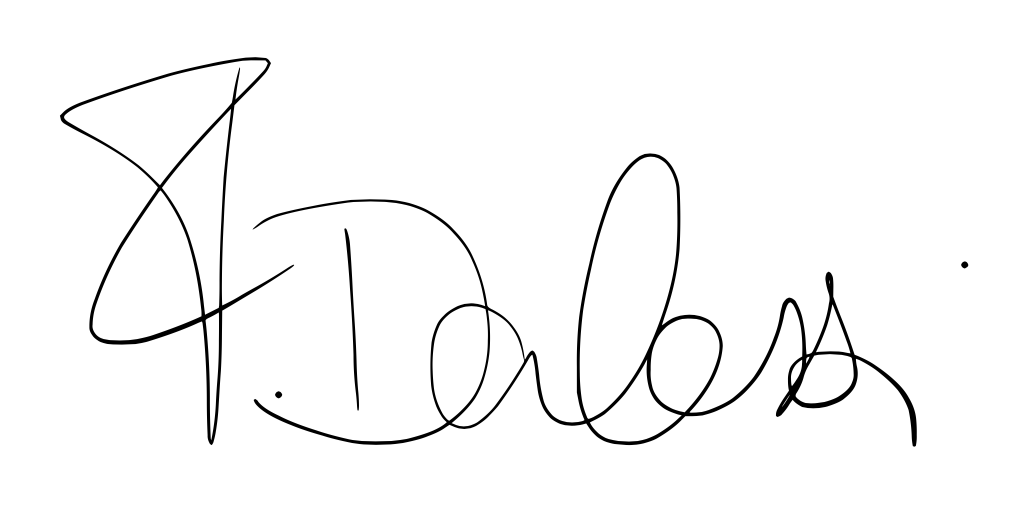
\includegraphics[height=1.2cm]{images/flavio_dalessi_signature.png}\\
        \large Flavio Dalessi
    \end{minipage}
    &
    \begin{minipage}{6cm}
    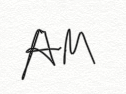
\includegraphics[height=1.2cm]{images/signatureAndreaMusso.png}\\
        \large Andrea Musso
    \end{minipage}
\end{tabular}
\\[2cm]
\begin{tabular}{@{}p{3.3cm}@{}p{6cm}@{}@{}p{6cm}@{}}
    \begin{minipage}{3cm}
    
    \end{minipage}
    &
    \begin{minipage}{6cm}
    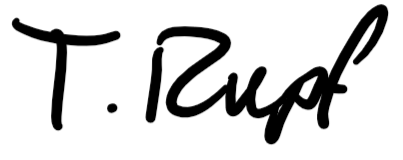
\includegraphics[height=1.2cm]{images/signature_thomas.png}\\
        \large Thomas Rupf
    \end{minipage}
    &
    \begin{minipage}{6cm}
        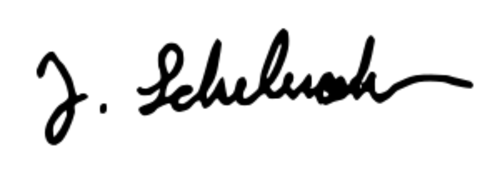
\includegraphics[height=1.2cm]{images/signature_julian.pdf}\\
        \large Julian Schuhmacher
    \end{minipage}
\end{tabular}
\\[2cm]
\begin{tabular}{@{}p{3.3cm}@{}p{6cm}@{}}
    \begin{minipage}{3cm}
    
    \end{minipage}
    &
    \begin{minipage}{6cm}
        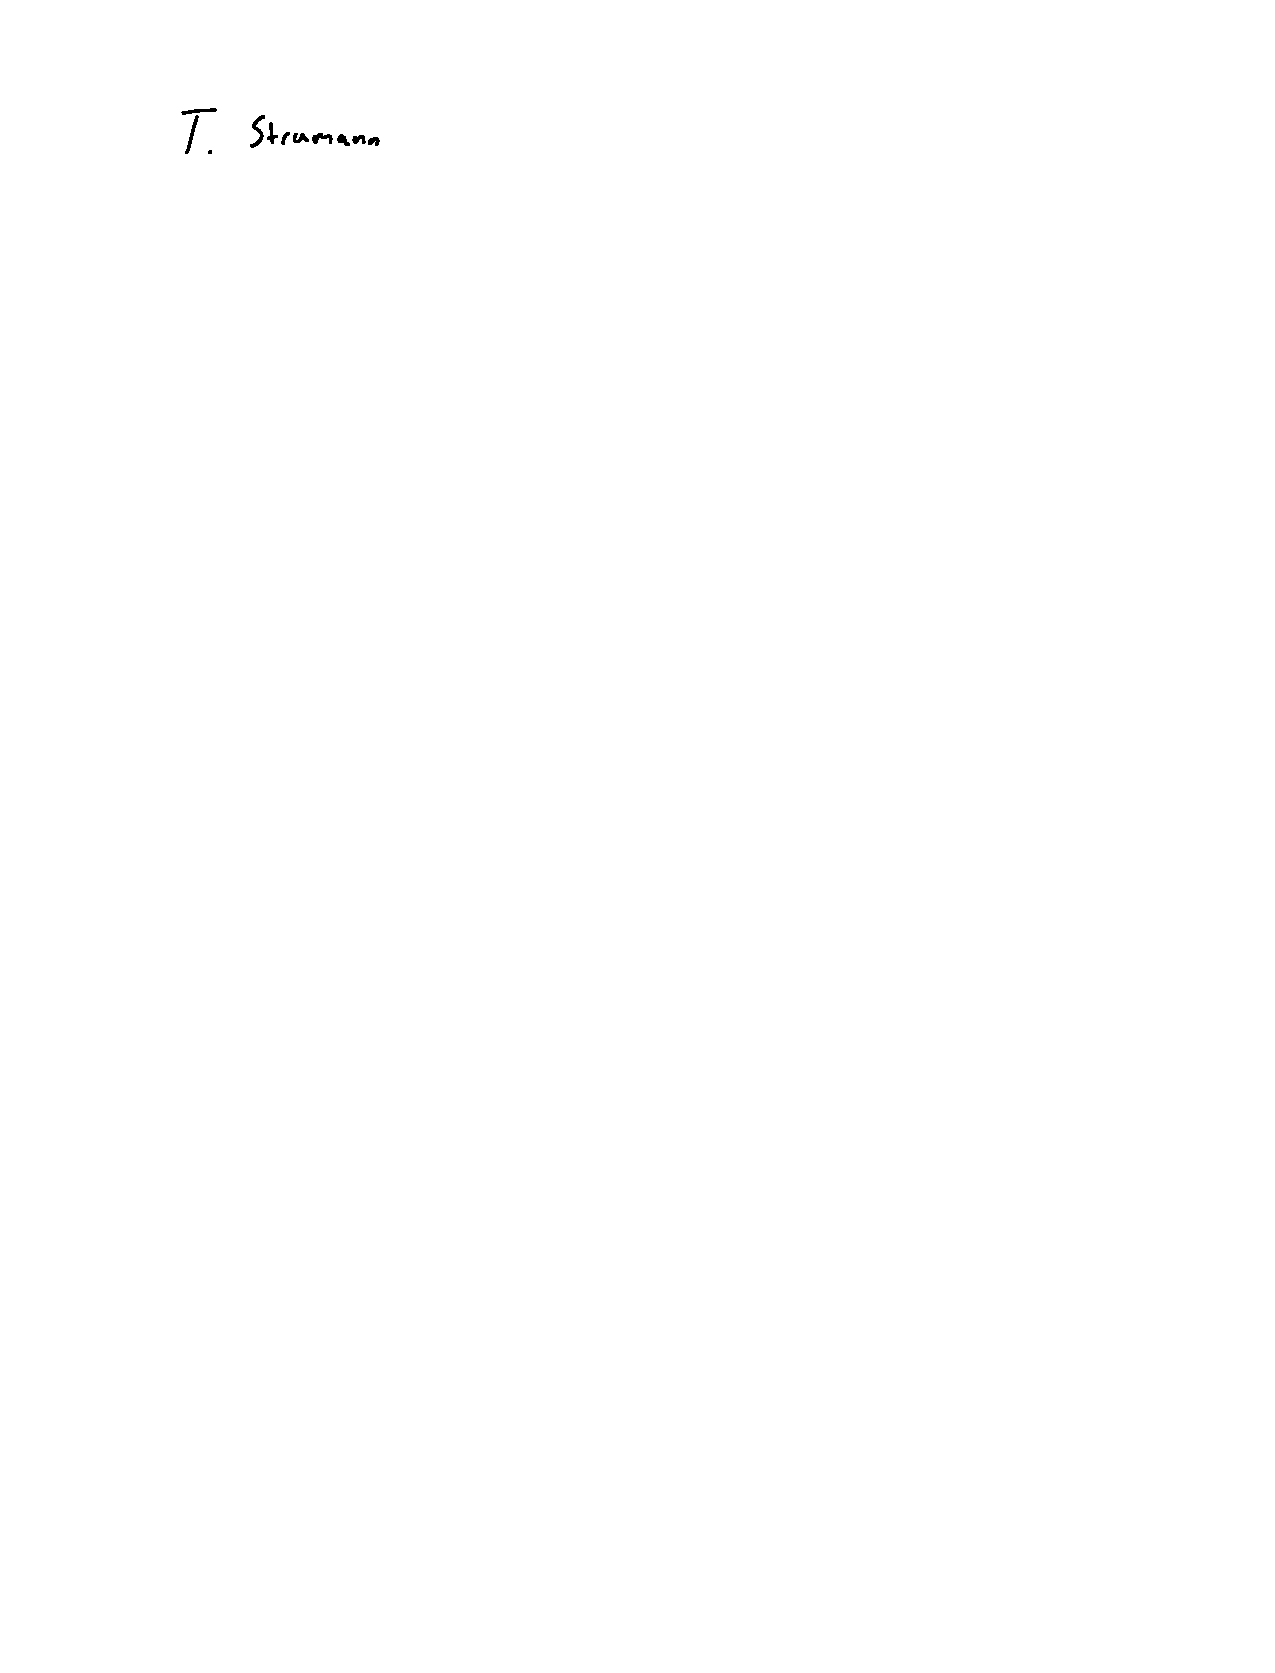
\includegraphics[height=1.2cm]{images/tristan_strumann_signature.pdf}\\
        \large Tristan Strumann
    \end{minipage}
\end{tabular}

\end{center}

\newpage

\subsection{Contributions to project}
The members of the group made the following contributions to the project:
\begin{enumerate}
    \item[Flavio] Model implementation; Research for comparison with other models, Model observation experiments; Model description in presentation.
    \item[Andrea] Read papers and directed project; Contribution to code in Agent, News and World classes and utils; Contribution to report writing.
    \item[Tristan] Model Animation; Graph structure experiment; Graph structure section in presentation and report
    \item[Thomas] Plotting and greedy algorithm implementation; Two news experiments and plots; contribution to multiple news section in presentation and report;
    \item[Julian] Model implementation; Model evaluation experiments; Repository maintenance; Model evaluation section in presentation and report
\end{enumerate}

% IMPORTANT
% you MUST include the ETH declaration of originality here; it is available for download on the course website or at http://www.ethz.ch/faculty/exams/plagiarism/index_EN; it can be printed as pdf and should be filled out in handwriting



\includepdf[]{declaration_originality.pdf}

\end{document}